\documentclass[12pt]{article}
\usepackage[utf8]{inputenc}
\usepackage[english]{babel}
\usepackage{amsmath}
\usepackage{amssymb}
\usepackage{geometry}
\usepackage{enumitem}
\usepackage{fancyhdr}
\usepackage{hyperref}
\usepackage{graphicx}
\usepackage{float} 
\usepackage{minted}
\usepackage{caption}
\usepackage{array}
\usepackage{longtable}
\usepackage{booktabs}
\usepackage{pgfplots} % Para gráficas
\pgfplotsset{compat=1.18}


\usepackage{tcolorbox}
\usepackage{hyperref}
\usepackage{fontawesome5}

% quita sangria
%\setlength{\parindent}{0pt}
%----

\usemintedstyle{tango}
\setminted{
    linenos,
    breaklines,
    fontsize=\footnotesize,
    bgcolor,
    numbersep=3pt,
    frame=single
}

% Cambiar estilo de números de línea
%\renewcommand{\theFancyVerbLine}{\textbf{\Large\arabic{FancyVerbLine}}}

%------
\geometry{margin=2.5cm}
\pagestyle{fancy}
\fancyhf{}
\rhead{practical session 1}
\lhead{parallel programming}
\cfoot{\thepage}

%---------------
\title{Practical Session 2}
\author{Juan Diego Collazos Mejia}
\date{\today}

%------------------------
\begin{document}

\maketitle

\section*{Ejercicio 1: Lectura}

\begin{itemize}
    \item \textbf{Producer and Consumer}
    \begin{center}
        \href{https://github.com/jucollas/parallel-programming/blob/main/practical-session-2/scripts/exercise-1/producer-consumer.c}{\faGithub\ \texttt{producer-consumer.c} in GitHub}
    \end{center}
    \begin{figure}[H]
        \centering
        \includegraphics[width=0.47\linewidth]{images/execution-producter-consumer.png}
        \caption{Execution Producter and Consumer}
        \label{fig:os}
    \end{figure}

    \item \textbf{Matrix x Vector}
    \begin{center}
        \href{https://github.com/jucollas/parallel-programming/blob/main/practical-session-2/scripts/exercise-1/matrix-vector-multiplication.c}{\faGithub\ \texttt{matrix-vector-multiplication.c} in GitHub}
    \end{center}
    \begin{figure}[H]
        \centering
        \includegraphics[width=0.37\linewidth]{images/execution-matrix-vector-mult.png}
        \caption{Execution matrix x vector}
        \label{fig:os}
    \end{figure}

    \item \textbf{Trapezoidal Rule}
    \begin{center}
        \href{https://github.com/jucollas/parallel-programming/blob/main/practical-session-2/scripts/exercise-1/trapezoidal-rule.c}{\faGithub\ \texttt{trapezoidal-rule.c} in GitHub}
    \end{center}
    \begin{figure}[H]
        \centering
        \includegraphics[width=0.8\linewidth]{images/execution-trapezoidal-rule.png}
        \caption{Execution Trapezoidal Rule}
        \label{fig:os}
    \end{figure}

    \item \textbf{Count Sort}
    \begin{center}
        \href{https://github.com/jucollas/parallel-programming/blob/main/practical-session-2/scripts/exercise-1/count-sort.c}{\faGithub\ \texttt{count-sort.c} in GitHub}
    \end{center}
    \begin{figure}[H]
        \centering
        \includegraphics[width=0.8\linewidth]{images/execution-count-sort.png}
        \caption{Execution Count Sort}
        \label{fig:os}
    \end{figure}
\end{itemize}

\section*{Ejercicio 2: Suma de un Arreglo Grande}

\subsection*{Pthread implementacion}

\begin{center}
    \href{https://github.com/jucollas/parallel-programming/blob/main/practical-session-2/scripts/exercise-2/adder_array_with_pthreand.cpp}{\faGithub \texttt{adder\_array\_with\_pthreand.cpp} in GitHub}
\end{center}
\begin{figure}[H]
    \centering
    \includegraphics[width=0.8\linewidth]{images/execution-sum-array-pthread.png}
    \caption{Execution SumArray Pthread}
    \label{fig:os}
\end{figure}

\begin{longtable}{>{\raggedright}p{2.5cm} >{\centering\arraybackslash}p{2cm} 
>{\centering\arraybackslash}p{3cm}}
\toprule
Size of array (N) & Threads & CPU Time (s) \\
\midrule
\endfirsthead
\toprule
Size of array (N) & Threads & CPU Time (s) \\
\midrule
\endhead
1e6 & 2 & 0.000948 \\
1e6 & 4 & 0.001389 \\
1e6 & 8 & 0.001574  \\
1e7 & 2 & 0.004705 \\
1e7 & 4 & 0.007255 \\
1e7 & 8 & 0.013487 \\
1e8 & 2 & 0.039386 \\
1e8 & 4 & 0.061709 \\
1e8 & 8 & 0.100795 \\
\bottomrule
\end{longtable}




\subsection*{OpenMP implementacion}

\begin{center}
    \href{https://github.com/jucollas/parallel-programming/blob/main/practical-session-2/scripts/exercise-2/adder_array_with_openMP.cpp}{\faGithub \texttt{adder\_array\_with\_openMP.cpp} in GitHub}
\end{center}
\begin{figure}[H]
    \centering
    \includegraphics[width=0.8\linewidth]{images/execution-sum-array-openmp.png}
    \caption{Execution SumArray Openmp}
    \label{fig:os}
\end{figure}

\begin{longtable}{>{\raggedright}p{2.5cm} >{\centering\arraybackslash}p{2cm} 
>{\centering\arraybackslash}p{3cm}}
\toprule
Size of array (N) & Threads & CPU Time (s) \\
\midrule
\endfirsthead
\toprule
Size of array (N) & Threads & CPU Time (s) \\
\midrule
\endhead
1e6 & 2 & 0.007395 \\
1e6 & 4 & 0.013883 \\
1e6 & 8 & 0.019693 \\
1e7 & 2 & 0.070266 \\
1e7 & 4 & 0.106531 \\
1e7 & 8 & 0.14082 \\
1e8 & 2 & 0.668011 \\
1e8 & 4 & 0.721224 \\
1e8 & 8 & 1.31289 \\
\bottomrule
\end{longtable}

\subsection*{Comparacion Implementaciones}

\begin{figure}[H]
\centering
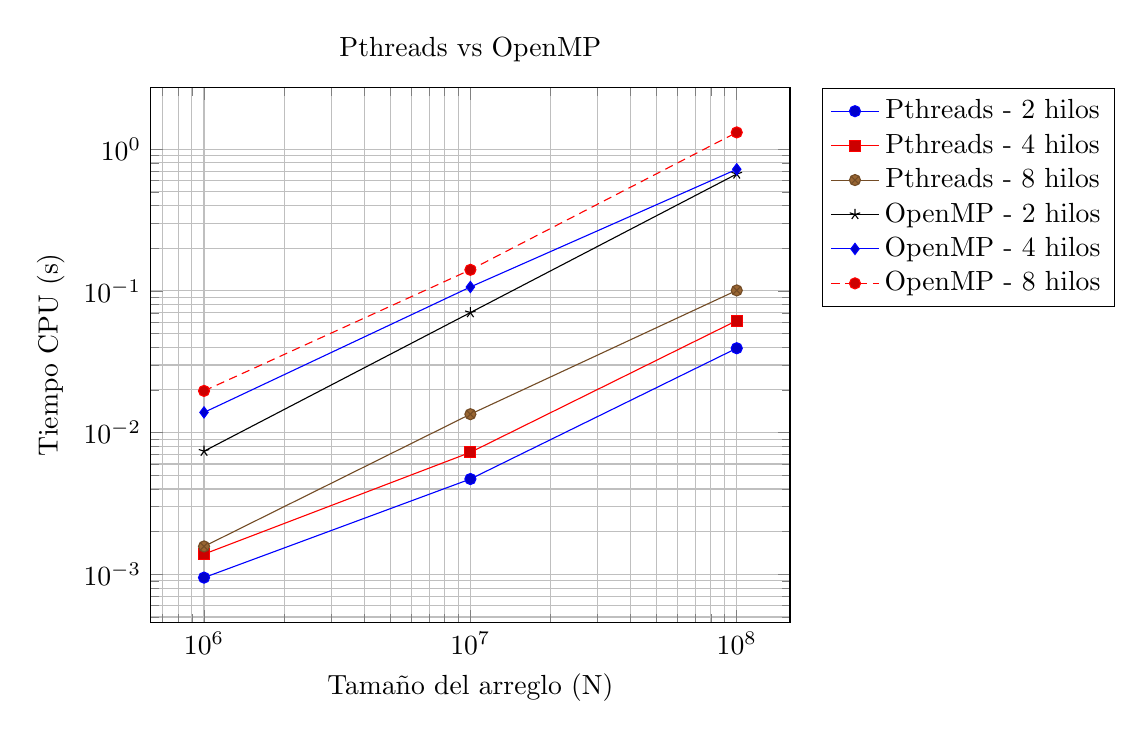
\begin{tikzpicture}
\begin{loglogaxis}[
    width=0.8\textwidth,
    xlabel={Tamaño del arreglo (N)},
    ylabel={Tiempo CPU (s)},
    title={Pthreads vs OpenMP},
    legend style={at={(1.05,1)}, anchor=north west},
    grid=both
]

% ==== PTHREADS ====
\addplot coordinates {(1e6,0.000948) (1e7,0.004705) (1e8,0.039386)};
\addlegendentry{Pthreads - 2 hilos}
\addplot coordinates {(1e6,0.001389) (1e7,0.007255) (1e8,0.061709)};
\addlegendentry{Pthreads - 4 hilos}
\addplot coordinates {(1e6,0.001574) (1e7,0.013487) (1e8,0.100795)};
\addlegendentry{Pthreads - 8 hilos}

% ==== OPENMP ====
\addplot coordinates {(1e6,0.007395) (1e7,0.070266) (1e8,0.668011)};
\addlegendentry{OpenMP - 2 hilos}
\addplot  coordinates {(1e6,0.013883) (1e7,0.106531) (1e8,0.721224)};
\addlegendentry{OpenMP - 4 hilos}
\addplot coordinates {(1e6,0.019693) (1e7,0.14082) (1e8,1.31289)};
\addlegendentry{OpenMP - 8 hilos}

\end{loglogaxis}
\end{tikzpicture}
\caption{Comparación del tiempo de ejecución entre Pthreads y OpenMP con distintos hilos}
\end{figure}

\section*{Conclusión}
A partir de los resultados obtenidos se observa que la implementación con \textbf{Pthreads} presenta tiempos de ejecución considerablemente menores frente a la implementación con \textbf{OpenMP}, para los tres tamaños de entrada analizados.\\

En particular, para un arreglo de $10^8$ elementos, \textbf{Pthreads} logra tiempos del orden de $0.04$ a $0.10$ segundos dependiendo de la cantidad de hilos, mientras que \textbf{OpenMP} requiere entre $0.66$ y $1.31$ segundos. Esto implica que, en este escenario, la eficiencia de \textbf{Pthreads} es entre 6 y 15 veces superior. \\

Además, se aprecia que al incrementar el número de hilos no siempre se obtiene una reducción proporcional del tiempo de ejecución. De hecho, tanto en \textbf{Pthreads} como en \textbf{OpenMP}, el incremento de hilos de $2$ a $8$ tiende a aumentar el tiempo de ejecución en lugar de disminuirlo, lo cual puede atribuirse a la \textit{sobrecarga de sincronización} y a la gestión de hilos. \\

En conclusión, la implementación con \textbf{Pthreads} resulta más eficiente para este problema específico de suma de arreglos, mientras que \textbf{OpenMP} muestra un mayor costo en términos de tiempo de CPU conforme aumenta el tamaño de entrada y el número de hilos.



\section*{Ejercicio 3: Multiplicación de Matrices}

\begin{center}
    \href{https://github.com/jucollas/parallel-programming/blob/main/practical-session-2/scripts/exercise-3/mult_matrix_parallel.cpp}{\faGithub \texttt{mult\_matrix\_parallel.cpp} in GitHub}
\end{center}
\begin{figure}[H]
    \centering
    \includegraphics[width=0.8\linewidth]{images/execution-matrix-mult.png}
    \caption{Execution MatrixMult}
    \label{fig:os}
\end{figure}





\end{document}

\begin{itemize}[left = 0pt]
    \item Describe the four Flynn Architecture Classifications. Explain why the MISD configuration has traditionally been thought of as non-sensible.\\
    $\blacktriangleright$ \\
    Flynn (1966) classified computer architectures according to the number of instruction streams and data streams they can handle simultaneously:
    \begin{enumerate}
        \item \textbf{SISD (Single Instruction, Single Data) }
        \begin{itemize}
            \item Traditional von Neumann architecture.
            \item A single processor executes one instruction stream on one data stream.
            \item Example: classic uniprocessor.
        \end{itemize}

        \item \textbf{SIMD (Single Instruction, Multiple Data)}
        \begin{itemize}
            \item  One control unit broadcasts the same instruction to multiple processing elements, each working on different data.
           \item Very efficient for vector/matrix operations, image/video processing.
           \item  Example: GPUs, vector processors.
        \end{itemize}

        \item \textbf{MISD (Multiple Instruction, Single Data)}
        \begin{itemize}
            \item Multiple instruction streams operate on the \textbf{same} data stream.
            \item Traditionally considered non-sensible because having several different instructions acting on the same piece of data rarely offers useful computation.
            \item However, some fault-tolerant systems use MISD-like redundancy (e.g., multiple processors computing the same result in different ways to detect errors).
        \end{itemize}

        \item \textbf{MIMD (Multiple Instruction, Multiple Data)}
        \begin{itemize}
            \item Multiple processors execute independent instruction streams on independent data streams.
            \item Most modern multiprocessors and multicore systems fall into this category.
            \item Example: multicore CPUs, distributed computing clusters.
        \end{itemize}
    \end{enumerate}
    \newpage
    $\blacktriangleright$ \textbf{Why MISD is Non-Sensible}
    \begin{itemize}
        \item The idea of having many instructions act on the same data point is not useful in practice for general-purpose computing.
        \item It wastes hardware resources because you could instead process different data (MIMD) or the same operation on different data (SIMD).
        \item Only niche applications like \textbf{fault tolerance} or \textbf{real-time control systems} justify MISD. 
    \end{itemize}

    \item One of the design goals of Instruction-Level Parallelism (ILP) was to make it transparent to the software layer; however, there are limitations as to how effective it is, and to what degree of aggressiveness or “look-ahead” it can be performed at. What are the causes of the limitations and how do they arise?\\
    $\blacktriangleright$ \\
    ILP tries to exploit parallelism *within a single program stream* by overlapping instruction execution (e.g., pipelining, superscalar execution, out-of-order execution).
    
    Limitations arise from:
    \begin{enumerate}
        \item \textbf{Data dependencies}
        \begin{itemize}
            \item True data dependence: instruction B needs the result of A.
            %\item Anti-dependence and output dependence complicate reordering.
        \end{itemize}

        \item  \textbf{Control dependencies}
        \begin{itemize}
            \item Branches make it hard to know which instructions should execute next.
            \item Branch prediction is imperfect.
        \end{itemize}

        \item  \textbf{Memory dependencies}
        \begin{itemize}
            \item Unknown whether two memory references alias (point to the same address).
        \end{itemize}
        \item \textbf{Hardware complexity}
        \begin{itemize}
            \item Aggressive ILP (large reorder buffers, speculation, register renaming) increases power, cost, and design difficulty.
            \item Diminishing returns: beyond a certain point, extra complexity doesn’t yield much more parallelism.
        \end{itemize}        
    \end{enumerate}

    \item What are the micro-architecture and  macro-architecture trends and HWdesign problems that have led to the need for programmers to explicitly express parallelism into their software?\\
    $\blacktriangleright$\\
    Over time, several hardware design issues forced programmers to take more responsibility for expressing parallelism:
    \begin{itemize} 
        \item End of frequency scaling (around mid-2000s): clock rates hit thermal and power walls.
        \item Limited ILP: hardware cannot “find” enough parallelism automatically in sequential programs.
        \item Rise of multicore CPUs and GPUs: parallel execution units are abundant, but require explicit parallel software.
        \item Memory wall: latency of memory access doesn’t scale like CPU speed; requires careful programmer-managed parallel memory access (tiling, blocking). 
    \end{itemize}


    \item What are some of the challenges associated with directly exposing the underlying hardware parallelism to the software layer and programmers?\\
    $\blacktriangleright$
    \begin{itemize}
        \item Complexity for programmers: writing parallel code is harder (synchronization, race conditions, deadlocks).
        \item Portability: code tuned for one parallel architecture may not map well to another.
        \item Debugging difficulties: nondeterministic execution due to interleavings.
        \item Load balancing: programmers must ensure even distribution of work across cores.
        \item Memory consistency models: different architectures have different visibility/ordering guarantees.
    \end{itemize}

    \item What is HyperThreading, and what, if anything, should software programmers do to leverage it as effectively as possible?\\
    $\blacktriangleright$\\
    Hyper-Threading (HT) is a technology developed by Intel that allows a single physical processor core to execute two threads at the same time.
    
    In simple terms:
    \begin{itemize}
        \item Each physical core presents itself to the operating system as two logical cores.
        \item This means that if you have a 4-core processor with Hyper-Threading, the operating system will see it as 8 logical processors.
    \end{itemize}

    \textbf{What programmers should do:}
    \begin{itemize}
        \item Write multithreaded code that can exploit more logical cores.
        \item Avoid excessive thread contention for shared resources (locks, memory bandwidth).
        \item Use standard parallel programming frameworks (e.g., OpenMP, TBB, pthreads) so the OS and runtime can map threads efficiently.
    \end{itemize}
\end{itemize}

\newpage

\section{Scripting Languages}

\subsection{Difference between output}

Execute the following 'C' programs, first interactively, then by
redirecting output to a file at the UNIX shell level with a "$>$".

\subsubsection*{Program 1}
\inputminted{cpp}{scripts/script-1.c}

\begin{figure}[h]
    \centering
    % Primera imagen (ocupa 45% del ancho de página)
    \begin{minipage}{0.45\textwidth}
        \centering
        \includegraphics[width=\linewidth]{images/interactive-script1.png}
        \caption{Interactively - script 1}
    \end{minipage}
    \hfill % espacio flexible entre imágenes
    % Segunda imagen
    \begin{minipage}{0.45\textwidth}
        \centering
        \includegraphics[width=\linewidth]{images/outfile-script1.png}
        \caption{Redirecting output to a file - script 1}
    \end{minipage}
\end{figure}

Explain the difference between the output observed on the terminal and that contained in the target piped file. \\
$\blacktriangleright$ 
The difference is caused by \textbf{buffering}.
\begin{itemize}
    \item  printf uses the C standard I/O library, which is line-buffered when writing to the terminal (it flushes on \n) but fully buffered when redirected to a file (data stays in memory until the program ends).
    \item write is a low-level system call: it writes immediately, without buffering.
\end{itemize}

So:
\begin{itemize}
    \item On the terminal, printf flushes right away (because of \n), so you see "Line 1 .." first.
    \item With redirection, printf waits in the buffer while write goes directly to the file, so "Line 2 " appears before "Line 1 ..".
\end{itemize}

\newpage

\subsubsection*{Program 2}

\inputminted{cpp}{scripts/script-2.c}

\begin{figure}[h]
    \centering
    % Primera imagen (ocupa 45% del ancho de página)
    \begin{minipage}{0.45\textwidth}
        \centering
        \includegraphics[width=\linewidth]{images/interactive-script2.png}
        \caption{Interactively - script 2}
    \end{minipage}
    \hfill % espacio flexible entre imágenes
    % Segunda imagen
    \begin{minipage}{0.45\textwidth}
        \centering
        \includegraphics[width=\linewidth]{images/outfile-script2.png}
        \caption{Redirecting output to a file - script 2}
    \end{minipage}
\end{figure}

Explain what has happened with the addition of the fflush system call. \\
$\blacktriangleright$ On the terminal there is no difference because stdout is line-buffered and the \n flushes the buffer, but with redirection fflush forces the buffer to be flushed, ensuring that "Line 1 ..." is written first and the sequential order in the file is preserved.

\subsection{The different execution order on different runs}

\subsubsection*{Program 3}
Improve and run the following 'C' program several times interactively.
\inputminted{cpp}{scripts/script-3.c}

\begin{figure}[h]
    \centering
    % Primera imagen (ocupa 45% del ancho de página)
    \begin{minipage}{0.45\textwidth}
        \centering
        \includegraphics[width=\linewidth]{images/outfile1-script3.png}
        \caption{Execution 1 - script 3}
    \end{minipage}
    \hfill % espacio flexible entre imágenes
    % Segunda imagen
    \begin{minipage}{0.45\textwidth}
        \centering
        \includegraphics[width=\linewidth]{images/outfile2-script3.png}
        \caption{Execution 2 - script 3}
    \end{minipage}
\end{figure}

Note the different execution order on different runs, Why? \\
\(\blacktriangleright\) The output order changes because after each \textbf{fork()}, both parent and child processes continue running concurrently from the same point. The operating system’s scheduler decides which process runs first, and this scheduling is non-deterministic. Therefore, the print statements can appear in different orders on each run.

\subsubsection*{Program 4}
Making the minor changes to program 3 above needed to get the code
below, execute the following 'C' program several times
interactively.

\inputminted{cpp}{scripts/script-4.c}

\begin{figure}[H]
    \centering
    % Primera imagen (ocupa 45% del ancho de página)
    \begin{minipage}{0.45\textwidth}
        \centering
        \includegraphics[width=\linewidth]{images/outfile1-script4.png}
        \caption{Execution 1 - script 4}
    \end{minipage}
    \hfill % espacio flexible entre imágenes
    % Segunda imagen
    \begin{minipage}{0.45\textwidth}
        \centering
        \includegraphics[width=\linewidth]{images/outfile2-script4.png}
        \caption{Execution 2 - script 4}
    \end{minipage}
\end{figure}

Explain how and why the order of the output from this program is
different from that of the after program.

\(\blacktriangleright\)
The use of wait(NULL) makes the output deterministic because the parent is forced to pause until its child finishes execution. As a result, each iteration always prints the child’s message first, followed by the parent’s message, in a fixed order.

\subsection{Encrypt and decrypt programs}

Create encrypt\_it and decrypt\_it programs using C, C++ and bash scripting language. Both receive two arguments: the rotation index and the phrase to be encrypted or decrypted.

%\inputminted{cpp}{scripts/cipher-cesar.cpp

\begin{center}
    \href{https://github.com/jucollas/parallel-programming/blob/main/practical-session-1/scripts/cfiles/cipher-cesar.cpp}{\faGithub\ \texttt{cipher-cesar.cpp} in GitHub}
\end{center}

\begin{itemize}
    \item  Encrypt "Aprendiendo Programación paralela".
    \begin{figure}[H]
        \centering
        \includegraphics[width=0.8\linewidth]{images/cipher-execute1.png}
        \caption{Execution 1 cipher-cesar}
        \label{fig:os}
    \end{figure}
    
    \item  Decrypt "Zú iolxgju Ikygx, latioutg!" with rotation 6.

    \begin{figure}[H]
        \centering
        \includegraphics[width=0.8\linewidth]{images/cipher-execute2.png}
        \caption{Execution 2 cipher-cesar}
    \end{figure}

    \item  Encrypt\_it with two different sets of arguments and redirect its output to two separate files and show the content.

    \begin{figure}[H]
        \centering
        \includegraphics[width=0.8\linewidth]{images/cipher-execute3.png}
        \caption{Execution 3 cipher-cesar}
    \end{figure}

    \begin{figure}[H]
        \centering
        \includegraphics[width=0.8\linewidth]{images/cipher-execute4.png}
        \caption{Execution 4 cipher-cesar}
    \end{figure}
    
    \item Decrypt the text processed after.
    \begin{figure}[H]
        \centering
        \includegraphics[width=0.8\linewidth]{images/cipher-execute5.png}
        \caption{Execution 5 cipher-cesar}
    \end{figure}

    \begin{figure}[H]
        \centering
        \includegraphics[width=0.8\linewidth]{images/cipher-execute6.png}
        \caption{Execution 6 cipher-cesar}
    \end{figure}
\end{itemize}

\newpage

Questions:
\begin{itemize}
    \item \textbf{Have you reached parallel code? Or parallel behavior?} \\
    \(\blacktriangleright\) These programs are sequential, not parallel. Each character is processed one after another.

    \item \textbf{Does the shell-script code perform parallelism or pipelining?} \\
    \(\blacktriangleright\) No, it is also sequential. Shell scripts can launch parallel processes using \texttt{\&} or pipelines \texttt{|}, but our encryption runs linearly.

    \item \textbf{But if script-based parallel programming is so easy, why bother with anything else?} \\ 
    \(\blacktriangleright\) Because:
    \begin{itemize}
        \item Scripts are limited in performance (slow, high overhead).
        \item Not suitable for fine-grained parallelism (e.g., character-level).
        \item Real parallel programming in C/C++ (with threads, OpenMP, MPI) gives better control, efficiency, and scalability.
    \end{itemize}
\end{itemize}

\section{POSIX Environment}

Another alternative to achieve basic parallelism is the POSIX
environment. This includes primitives to manage processes and
pthreads. This environment is readily available and widely supported
by modern Operating Systems.\\

Real-world applications using fork(), kill(), exit(), among other
primitives to manipulate signals, file descriptors, shared memory
segments, and any number of other resources.

\begin{itemize}
\item Write a C program that uses fork to create a child process.
\item The child process should calculate the sum of all numberswithin a given range. Meanwhile, the parent process waits for the child to finish. Once the child completes the calculation, it sends the result to the parent using a pipe, and the parent prints the result. (sum.c)

\begin{center}
    \href{https://github.com/jucollas/parallel-programming/blob/main/practical-session-1/scripts/cfiles/sum.c}{\faGithub\ \texttt{sum.c} in GitHub}
\end{center}

%\inputminted{cpp}{scripts/sum.c}

\begin{figure}[H]
    \centering
    \includegraphics[width=0.8\linewidth]{images/sum-execute1.png}
    \caption{Execution 1 sum.c}
\end{figure}

\item Improve the code and use the fork primitive to create (n/3) child processes (adder.c) for a input of length (n)
\item Modifies the program to receive the a list of numbers from standard input

\begin{center}
    \href{https://github.com/jucollas/parallel-programming/blob/main/practical-session-1/scripts/cfiles/adder.c}{\faGithub\ \texttt{adder.c} in GitHub}
\end{center}

\begin{figure}[H]
    \centering
    \includegraphics[width=0.8\linewidth]{images/adder-execute1.png}
    \caption{Execution 1 adder.c}
\end{figure}


\item Create a program to generate n number randomly generated and print in standard output (randomizer.c)

\begin{center}
    \href{https://github.com/jucollas/parallel-programming/blob/main/practical-session-1/scripts/cfiles/randomizer.c}{\faGithub\ \texttt{randomizer.c} in GitHub}
\end{center}

\begin{figure}[H]
    \centering
    \includegraphics[width=0.8\linewidth]{images/randomizer-execute1.png}
    \caption{Execution 1 ramdomizer.c}
\end{figure}

\item Pipeline randomizer and adder programs
\begin{figure}[H]
    \centering
    \includegraphics[width=0.8\linewidth]{images/randomizer-and-adder-execute1.png}
    \caption{Execution 1 ramdomizer and adder}
\end{figure}

\end{itemize}

Questions:
\begin{itemize}
    \item Child processes run in parallel mode? Or concurrently? Why?\\
    \(\blacktriangleright\) Child processes run concurrently, and if the system has multiple CPU cores, they can run in parallel. This is because \textbf{fork()} creates independent processes scheduled by the operating system, which may interleave them on one core or truly execute them simultaneously on multiple cores.
    
    \item Is the running time equal for sum and adder programs? Which is faster? Why?

    \(\blacktriangleright\)
    \textbf{The running time is not equal}.
    \begin{itemize}
        \item On a single-core system, the sum program is usually faster because it avoids the overhead of multiple processes and IPC.
        \item On a multi-core system, the adder program can be faster because the workload is divided among several child processes that may execute in parallel, reducing the effective computation time.
    \end{itemize}
\item Do parent and child processes use shared memory? Is it
important?\\
\(\blacktriangleright\) By default, parent and child processes do not share memory. Each has its own private address space after \textbf{fork()}. Communication requires Inter-Process Communication (IPC) mechanisms such as pipes (used in your code). This is important because it prevents accidental interference between processes but introduces overhead compared to shared memory approaches.
\end{itemize}

\subsection{Programming with threads}
A programming model that allows multiple threads to exist in a
single process, sharing the same memory space and a Thread is a
single sequence of programming instructions.
A process may create many threads. In Linux terminology, the main
thread is called the leader. We can call all the other created
threads followers. All the followers must have the same PID and PPID
as the leader. They will however have mutually distinct TIDs. The
followers should share almost everything (as in pthread) except the
stack.
\begin{itemize}
    \item Write a program to create two matrices, A and B, of sizes 40x40, which only take binary inputs 0 and 1.
    \item Create two threads: a thread will compute the summation of the two matrices and the other will compute their difference parallely. There will be one main thread which will wait for the two parallel threads to complete their task and it will compute the multiplication of the two previously obtained outputs and print the final output.

    \begin{center}
    \href{https://github.com/jucollas/parallel-programming/blob/main/practical-session-1/scripts/cfiles/matrices-threads.c}{\faGithub\ \texttt{matrices-threads.c} in GitHub}
    \end{center}
\end{itemize}
\end{document}